\documentclass[preprint,12pt]{elsarticle}

\usepackage{amsmath,amssymb,amsfonts}
\usepackage{amsthm}
\usepackage{graphicx}
\usepackage{booktabs}
\usepackage{multirow}
\usepackage{algorithm}
\usepackage{algorithmic}
\usepackage{hyperref}
\usepackage{xcolor}

\newtheorem{proposition}{Proposition}

\journal{Applied Mathematics and Computation}

\begin{document}

\begin{frontmatter}

\title{Spatiotemporal spectral derivatives with forward stepwise BIC for robust partial differential equation discovery}

\author[1]{Fuchang Wang\corref{cor1}}
\author[2]{Huirong Cao}

\address[1]{School of Science, Emergency Management University, No. 465 College Road, Sanhe, Hebei 065201, China}
\address[2]{School of Science, Langfang Normal University, No. 100 Ai-min Road, Langfang, Hebei 065000, China}

\cortext[cor1]{Corresponding author. Tel.: +86-xxx-xxxx-xxxx; email: wangfuchang@cidp.edu.cn}

\begin{abstract}
Data-driven discovery of partial differential equations (PDEs) from noisy data is limited by two factors: inaccurate derivative computation and threshold-sensitive sparse regression. We propose a spectral weak formulation that addresses both. Spatial and temporal derivatives are computed through a single two-dimensional Fourier transform over the space-time domain, which resolves non-periodic traveling-wave solutions where spatial-only spectral methods fail. The regression is formulated in weak form by integrating the PDE residual against localized Gaussian test functions, suppressing high-frequency noise in high-order derivatives. Candidate terms are normalized to unit $\ell_2$ norm, and forward stepwise selection with the Bayesian information criterion determines sparsity automatically without threshold tuning. On the MDBench benchmark, the method recovers the Burgers equation at all noise levels, achieves exact recovery of KdV and Kuramoto--Sivashinsky at moderate noise, and recovers the non-periodic advection equation exactly where finite-difference baselines fail. It is 10--20 times faster than Weak SINDy on periodic problems.
\end{abstract}

\begin{keyword}
PDE discovery \sep spectral methods \sep sparse regression \sep Bayesian information criterion \sep non-periodic problems
\end{keyword}

\end{frontmatter}

\section{Introduction}
\label{sec:intro}

Data-driven discovery of partial differential equations (PDEs) from simulation or experimental data offers a way to extract interpretable governing laws directly from measurements. The sparse identification of nonlinear dynamics (SINDy) framework \cite{brunton2016discovering,rudy2017data} formulates this as a sparse regression problem: build a library of candidate terms (polynomials and spatial derivatives), then find a sparse coefficient vector $\boldsymbol{\xi}$ satisfying $\mathbf{u}_t \approx \Theta(u)\boldsymbol{\xi}$. Despite rapid progress, two bottlenecks remain for practical deployment.

First, derivative computation from noisy data is ill-conditioned. Finite differences amplify high-frequency noise as their order grows, making fourth-order derivatives such as $u_{xxxx}$ unreliable. Spectral methods achieve exponential convergence but assume periodic boundaries; on non-periodic data they suffer Gibbs ringing. The exponentially filtered spectral derivatives of Schaeffer and McCalla \cite{schaeffer2017learning} suppress but do not eliminate this ringing.

Second, the standard solver---sequentially thresholded least squares (STLSQ)---requires a manually chosen threshold. This threshold varies with noise level and problem, and a poor choice either retains spurious terms or drops true ones. Weak SINDy \cite{messenger2021weak} improves noise robustness by integrating against test functions, but still relies on threshold tuning. SR3 \cite{kaheman2020sindypi} and related relaxations \cite{champion2020unified,gurevich2019robust} improve convergence but do not automate model selection.

We address both bottlenecks with three connected ideas.

\begin{enumerate}
\item \textbf{Spatiotemporal spectral derivatives.} Instead of transforming space at each time step independently, we apply a single two-dimensional Fourier transform over the joint space-time grid. For a traveling wave $u(x,t)=f(x-ct)$, the spectrum concentrates along the line $k_t=-ck_x$ (Proposition~\ref{prop:traveling}), while boundary-induced Gibbs noise spreads isotropically. A 2D filter separates the two, enabling accurate derivatives on non-periodic traveling-wave solutions that defeat spatial-only spectral methods.

\item \textbf{Spectral weak formulation.} The regression is set in weak form: both sides of the PDE are integrated against compactly supported Gaussian test functions before regression. This integration acts as an additional low-pass filter on high-order derivatives. We prove a spectral convergence error bound (Proposition~\ref{prop:spectral}).

\item \textbf{Normalized forward stepwise BIC.} Each candidate term is scaled to unit $\ell_2$ norm, and forward stepwise selection with the Bayesian information criterion \cite{schwarz1978estimating} chooses the support automatically. No threshold grid search is needed. We prove support consistency under standard conditions (Proposition~\ref{prop:bic}).
\end{enumerate}

The key numerical evidence is a control-variable comparison: we implement spatial-only spectral derivatives with the same exponential filter and BIC selection, then replace only the transform with our spatiotemporal version. On the non-periodic advection equation, the spatial-only version fails completely (0/1 true terms) while the spatiotemporal version recovers both terms exactly. On periodic problems, accuracy is comparable to Weak SINDy at 10--20$\times$ lower cost. Experiments cover Burgers, KdV, Kuramoto--Sivashinsky, and three higher-dimensional problems on the MDBench benchmark \cite{ziaei2025mdbench}.

The paper is organized as follows. Section~\ref{sec:related} reviews related work. Section~\ref{sec:method} presents the methodology. Section~\ref{sec:experiments} reports experiments. Section~\ref{sec:discussion} discusses limitations. Section~\ref{sec:conclusion} concludes.
\section{Related work}
\label{sec:related}

\subsection{Sparse regression for PDE discovery}

The SINDy framework \cite{rudy2017data} formulates PDE discovery as a sparse regression problem. Given a library of candidate terms $\Theta(u) \in \mathbb{R}^{N \times P}$ and the time derivative $\mathbf{u}_t \in \mathbb{R}^N$, the goal is to find a sparse coefficient vector $\boldsymbol{\xi} \in \mathbb{R}^P$ such that $\mathbf{u}_t \approx \Theta(u)\boldsymbol{\xi}$. The STLSQ algorithm solves this by iteratively: (1) solving a ridge regression, (2) thresholding small coefficients to zero, and (3) re-solving the least squares problem on the remaining support.

Several variants improve robustness. The sparse relaxed regularized regression (SR3) method \cite{kaheman2020sindypi} introduces a relaxation variable. This decouples the sparsity penalty from the data fidelity term and improves convergence. Champion et al. \cite{champion2020unified} proposed a unified sparse optimization framework that integrates physics-informed constraints. The weak SINDy formulation \cite{messenger2021weak} replaces pointwise derivatives with integrals against test functions. This significantly reduces noise sensitivity. Gurevich et al. \cite{gurevich2019robust} proposed a robust and optimal sparse regression for nonlinear PDE models that combines weak-form integration with optimal weighting. Messenger et al. \cite{messenger2022online} extended the weak-form approach to an online setting that processes snapshots sequentially. Fasel et al. \cite{fasel2022ensemble} introduced Ensemble-SINDy, which uses bootstrapping to improve recovery in the low-data, high-noise regime. Trajectory-based methods \cite{kaptanoglu2022pde} use multiple initial conditions to improve identifiability. Chen et al. \cite{chen2021physics} combined physics-informed learning with symbolic regression for scarce data regimes. The open-source PySINDy package \cite{kaptanoglu2022pysindy} provides implementations of these methods and is used as the baseline framework in this work.

\subsection{Spectral methods for derivative computation}

Spectral methods offer exponential convergence for smooth functions \cite{canuto2006spectral}. They are natural candidates for derivative computation in PDE discovery. Schaeffer and McCalla \cite{schaeffer2017learning} used Fourier spectral derivatives with exponential filtering to compute high-order derivatives robustly. Their method applies the transform spatially at each time step independently. It therefore inherits the periodic boundary assumption. For non-periodic data, the exponential filter suppresses but does not eliminate Gibbs ringing. The present work instead computes a single two-dimensional transform over the space-time domain. This exploits temporal correlation to separate boundary artifacts from the signal, as discussed in Section \ref{sec:theory}.

To address non-periodic problems, Chebyshev spectral methods have been proposed \cite{kopriva2009implementing}. These require data sampled on Chebyshev--Gauss--Lobatto grids. Experimental data rarely use such grids. Windowing techniques can reduce Gibbs phenomena but introduce additional errors.

\subsection{Model selection in sparse regression}

The choice of sparsity level is critical in sparse regression. Information criteria such as the Akaike information criterion (AIC) and the Bayesian information criterion (BIC) \cite{schwarz1978estimating} provide principled ways to select model complexity. Forward stepwise regression adds features one at a time based on their contribution to model fit. Combined with an information criterion for stopping, it offers a computationally efficient alternative to $\ell_1$ regularization. It also provides automatic model selection.

\section{Methodology}
\label{sec:method}

\subsection{Problem formulation}

Consider a spatio-temporal dataset $u(x_j, t_n)$ for $j = 1, \ldots, N_x$ and $n = 1, \ldots, N_t$, sampled from a PDE of the form
\begin{equation}
u_t = \mathcal{N}(u, u_x, u_{xx}, \ldots, x, t),
\end{equation}
where $\mathcal{N}$ is a (typically nonlinear) function involving polynomials of $u$ and its spatial derivatives. The goal is to identify the active terms in $\mathcal{N}$ and their coefficients from the data.

Following the SINDy framework, we construct a library of candidate terms
\begin{equation}
\Theta(u) = [\mathbf{1}, u, u^2, \ldots, u_x, u_{xx}, \ldots, u u_x, u^2 u_x, \ldots],
\end{equation}
and seek a sparse coefficient vector $\boldsymbol{\xi}$ such that
\begin{equation}
\mathbf{u}_t = \Theta(u) \boldsymbol{\xi} + \boldsymbol{\epsilon},
\end{equation}
where $\mathbf{u}_t$ is the vectorized time derivative and $\boldsymbol{\epsilon}$ represents noise and modeling errors.

\subsection{Spatiotemporal spectral derivatives}
\label{sec:spacetime}

A key challenge in PDE discovery is computing spatial derivatives accurately from noisy data. Standard approaches use finite differences or spatial-only spectral methods. Finite differences introduce truncation errors $O(\Delta x^p)$ that grow with derivative order. Spatial-only spectral methods assume periodicity in $x$ and fail for non-periodic solutions.

We propose computing derivatives in the combined space-time domain. Define the two-dimensional discrete Fourier transform (DFT) of $u$ as
\begin{equation}
\hat{u}(k_x, k_t) = \sum_{j=1}^{N_x} \sum_{n=1}^{N_t} u(x_j, t_n) e^{-i(k_x x_j + k_t t_n)},
\end{equation}
where $k_x$ and $k_t$ are the spatial and temporal frequency vectors. The spatial derivative of order $m$ is
\begin{equation}
\partial_x^m u = \mathcal{F}^{-1}\left[(i k_x)^m \hat{u}(k_x, k_t) \cdot \phi(k_x, k_t)\right],
\end{equation}
and the time derivative is
\begin{equation}
u_t = \mathcal{F}^{-1}\left[i k_t \hat{u}(k_x, k_t) \cdot \phi(k_x, k_t)\right],
\end{equation}
where $\phi(k_x, k_t)$ is a low-pass filter that suppresses high-frequency noise.

We use a separable exponential filter applied independently to each frequency dimension:
\begin{equation}
\phi(k_x, k_t) = \phi_1(k_x) \cdot \phi_1(k_t), \qquad
\phi_1(k) = \begin{cases}
1, & |k| \le k_c, \\
\exp\!\left[-\alpha \left(\frac{|k|-k_c}{k_{\max}-k_c}\right)^p\right], & |k| > k_c,
\end{cases}
\end{equation}
where $k_c$ is the cutoff frequency, $k_{\max}$ is the Nyquist frequency, $p$ is the filter order, and $\alpha = -\ln(\epsilon_{\text{tol}})$ with $\epsilon_{\text{tol}} = 10^{-12}$. We use $p = 8$ and $k_c = 0.6 k_{\max}$ as defaults.

The spatiotemporal approach has a critical advantage. The two-dimensional Fourier transform implicitly handles the temporal evolution of the solution. For non-periodic problems such as the advection equation, the solution profile translates in time. The spatiotemporal spectrum captures this traveling wave structure. The filter then suppresses the Gibbs artifacts that would appear in a spatial-only transform. This mechanism is analyzed theoretically in Section~\ref{sec:theory} and demonstrated empirically in Section~\ref{sec:experiments}.

\subsection{Theoretical analysis}
\label{sec:theory}

We now provide theoretical justification for the key components of the proposed method.

\subsubsection{Spectral accuracy of spatiotemporal derivatives}

\begin{proposition}[Spectral convergence]
\label{prop:spectral}
Let $u(x,t) \in C^\infty([0,L_x]\times[0,L_t])$ be a smooth function with Fourier coefficients $\hat{u}(k_x,k_t)$ decaying faster than any polynomial: for every $q>0$, there exists $C_q>0$ such that $|\hat{u}(k_x,k_t)| \le C_q (1+|k_x|+|k_t|)^{-q}$. Then the spatiotemporal spectral derivative of order $m$ satisfies
\begin{equation}
\|\partial_x^m u - \mathcal{D}_x^m u_N\|_\infty \le C_{m,q} N_x^{-q} + C_\phi \epsilon_{\mathrm{tol}},
\end{equation}
where $\mathcal{D}_x^m$ is the discrete spectral derivative operator, $N_x$ is the number of spatial grid points, and $C_\phi$ depends on the filter parameters.
\end{proposition}

\begin{proof}
Let $K_N = \{(k_x,k_t): |k_x|\le N_x/2,\; |k_t|\le N_t/2\}$ denote the retained frequency set. The discrete filtered derivative is
\begin{equation}
\mathcal{D}_x^m u_N(x,t) = \sum_{(k_x,k_t)\in K_N} (ik_x)^m \phi(k_x,k_t)\,\hat{u}(k_x,k_t)\,e^{i(k_x x+k_t t)}.
\end{equation}
The exact derivative is $\partial_x^m u = \sum_{k_x,k_t} (ik_x)^m \hat{u}(k_x,k_t) e^{i(k_x x+k_t t)}$. By the triangle inequality,
\begin{equation}
\|\partial_x^m u - \mathcal{D}_x^m u_N\|_\infty \le E_{\mathrm{trunc}} + E_{\mathrm{filter}},
\end{equation}
where the two terms are bounded separately.

\textit{Truncation error.} Dropping modes outside $K_N$ gives
\begin{equation}
E_{\mathrm{trunc}} \le \sum_{(k_x,k_t)\notin K_N} |k_x|^m |\hat{u}(k_x,k_t)|.
\end{equation}
Using the decay assumption $|\hat{u}(k_x,k_t)|\le C_q(1+|k_x|+|k_t|)^{-q}$, the sum over $k_t$ yields $\sum_{k_t}(1+|k_x|+|k_t|)^{-q}\le C'_q(1+|k_x|)^{1-q}$ for $q>2$. Therefore
\begin{equation}
E_{\mathrm{trunc}} \le C_q C'_q \sum_{|k_x|>N_x/2} |k_x|^{m-q+1} \le C_{m,q}\, N_x^{m-q+2},
\end{equation}
which is $O(N_x^{-r})$ for any $r>0$ by choosing $q>m+r+2$. This is spectral convergence.

\textit{Filter error.} Within $K_N$, the filter satisfies $1-\phi(k_x,k_t)\le \epsilon_{\mathrm{tol}}$ because $\phi\ge 1-\epsilon_{\mathrm{tol}}$ by construction of the exponential filter. Thus
\begin{equation}
E_{\mathrm{filter}} \le \sum_{(k_x,k_t)\in K_N} |k_x|^m |1-\phi|\,|\hat{u}| \le \epsilon_{\mathrm{tol}} \sum_{k_x,k_t} |k_x|^m |\hat{u}| \le \epsilon_{\mathrm{tol}}\,\|\partial_x^m u\|_{L^1},
\end{equation}
where the last step follows from the Fourier inversion formula and the triangle inequality. Setting $C_\phi=\|\partial_x^m u\|_{L^1}$ completes the proof.
\end{proof}

This result contrasts with finite difference methods, whose $m$-th order derivative error is $O(\Delta x^p)$ for a $p$-th order scheme, requiring increasingly fine grids for high-order derivatives.

\subsubsection{Traveling wave solutions and non-periodic problems}

\begin{proposition}[Traveling wave exactness]
\label{prop:traveling}
Let $u(x,t) = f(x - ct)$ be a traveling wave solution with speed $c$, where $f$ is smooth and compactly supported within the spatial domain. Then the spatiotemporal Fourier transform satisfies
\begin{equation}
\hat{u}(k_x, k_t) = \hat{f}(k_x) \cdot \delta(k_t + c k_x),
\end{equation}
where $\delta$ denotes the Dirac distribution. Consequently, the spectral energy concentrates along the line $k_t = -c k_x$ in the frequency plane. The two-dimensional low-pass filter $\phi(k_x,k_t)$ preserves this energy. It suppresses the Gibbs artifacts that arise from the spatial discontinuity at the domain boundary.
\end{proposition}

\begin{proof}
Substituting $u(x,t)=f(x-ct)$ into the Fourier transform gives
$\hat{u}(k_x,k_t) = \int\int f(x-ct) e^{-i(k_x x + k_t t)} dx dt$.
Changing variables $\xi = x-ct$ yields $\hat{u}(k_x,k_t) = \hat{f}(k_x) \int e^{-i(k_t + c k_x)t} dt = 2\pi \hat{f}(k_x) \delta(k_t + c k_x)$.
Thus all spectral energy lies on the characteristic line $k_t = -ck_x$. The spatial-only transform $\hat{f}(k_x)$ suffers from Gibbs ringing because $f$ is non-periodic on $[0,L_x]$, but in the spatiotemporal domain, the energy is concentrated along a one-dimensional manifold, and the two-dimensional filter can suppress the boundary-induced high-frequency components without distorting the signal along the characteristic direction.
\end{proof}

Proposition \ref{prop:traveling} explains why the spatiotemporal approach succeeds on the advection equation where spatial-only spectral methods fail. The traveling wave structure is naturally represented in the two-dimensional frequency domain. The Gibbs artifacts are separable from the signal.

This is a key distinction from spatial-only spectral methods. A spatial-only transform computes $\hat{u}(k_x) = \int u(x,t) e^{-ik_x x} dx$ at each time slice independently. For a non-periodic traveling wave, each slice exhibits Gibbs ringing at the boundaries. The ringing contaminates the derivative computation at every time step. In contrast, the spatiotemporal transform exploits the correlation across time. The signal energy concentrates along a one-dimensional manifold in the 2D frequency plane. The boundary-induced noise spreads isotropically in frequency space. A 2D low-pass filter can therefore remove the noise while preserving the signal along the characteristic direction. This mechanism is not available to spatial-only methods.

\subsubsection{Consistency of BIC model selection}

\begin{proposition}[BIC consistency]
\label{prop:bic}
Consider the linear model $\mathbf{y} = \Theta \boldsymbol{\xi}^* + \boldsymbol{\epsilon}$, where $\boldsymbol{\epsilon} \sim \mathcal{N}(0,\sigma^2 I_N)$, the true support $S^* = \{j: \xi_j^* \neq 0\}$ has size $s^*$, and the design matrix $\Theta$ satisfies the restricted eigenvalue condition with constant $\lambda_{\min} > 0$. If the minimum nonzero coefficient satisfies $\min_{j \in S^*} |\xi_j^*| > C \sqrt{\sigma^2 s^* \log N / N}$ for some constant $C$, then the BIC criterion selects the true model with probability tending to one as $N \to \infty$:
\begin{equation}
\mathbb{P}(\hat{S}_{\mathrm{BIC}} = S^*) \to 1 \quad \text{as } N \to \infty.
\end{equation}
\end{proposition}

\begin{proof}
Write $\mathrm{BIC}(S) = N\log(\hat{\sigma}_S^2)+|S|\log N$ with $\hat{\sigma}_S^2=\mathrm{RSS}(S)/N$. We compare any candidate model $S$ against the true model $S^*$ in two cases.

\textit{Overfitting ($S\supset S^*$, $|S|=s^*+k$).} The extra $k$ variables fit only noise. Under the restricted eigenvalue condition, the RSS reduction from adding $k$ noise variables is $O_p(k)$ uniformly. Hence $\hat{\sigma}_S^2 = \hat{\sigma}_{S^*}^2 - O_p(k/N)$, and
\begin{equation}
\mathrm{BIC}(S)-\mathrm{BIC}(S^*) = N\log\!\left(1-\frac{O_p(k/N)}{\hat{\sigma}_{S^*}^2}\right)+k\log N = -O_p(k)+k\log N > 0
\end{equation}
with probability tending to one, since $\log N\to\infty$.

\textit{Underfitting ($S\not\supset S^*$).} At least one true variable with coefficient $\xi_j^*$ is omitted. The restricted eigenvalue condition gives $\mathrm{RSS}(S)-\mathrm{RSS}(S^*)\ge \lambda_{\min} N (\xi_j^*)^2$ for the omitted component. Under the minimum coefficient condition $|\xi_j^*|>C\sqrt{\sigma^2 s^*\log N/N}$, this gap is $\Omega(\log N)$, and in fact $\Theta(N)$ when the omitted coefficient is $O(1)$. Thus
\begin{equation}
\mathrm{BIC}(S)-\mathrm{BIC}(S^*) = N\log\!\left(1+\frac{\Omega(\log N)}{N\hat{\sigma}_{S^*}^2}\right)-k\log N = \Omega(\log N)-O(\log N)>0
\end{equation}
for sufficiently large $N$.

Since every overfitting and underfitting model has strictly larger BIC than $S^*$, the global BIC minimizer is $S^*$. The forward stepwise algorithm is a greedy search: at each step it adds the variable that most reduces BIC. The minimum coefficient condition ensures that every true variable produces a BIC decrease when added, so the greedy path includes $S^*$ before stopping. Therefore $\hat{S}_{\mathrm{BIC}}=S^*$ with probability tending to one.
\end{proof}

Proposition \ref{prop:bic} justifies the use of BIC for model selection in our framework: as the number of data points increases (which is typical for PDE data on fine grids), BIC reliably identifies the correct sparse set of terms. The forward stepwise algorithm provides an efficient greedy approximation to the exhaustive BIC optimization.

\subsection{Feature normalization}
\label{sec:norm}

The candidate terms in $\Theta(u)$ can have vastly different magnitudes due to the polynomial and derivative factors. For example, $u^2$ may be orders of magnitude larger than $u_{xxxx}$ for a smooth solution. This scale imbalance causes standard sparse regression algorithms to favor large-magnitude terms and discard small-magnitude ones, even when they are physically important.

We address this by normalizing each feature to unit $\ell_2$ norm:
\begin{equation}
\tilde{\Theta}_j = \frac{\Theta_j}{\|\Theta_j\|_2}, \quad j = 1, \ldots, P,
\end{equation}
where $\Theta_j$ is the $j$-th column of $\Theta$. After solving the sparse regression on the normalized features $\tilde{\Theta}$, the coefficients are rescaled back:
\begin{equation}
\xi_j = \frac{\tilde{\xi}_j}{\|\Theta_j\|_2}.
\end{equation}
This normalization ensures that all candidate terms are treated equally during the model selection process, regardless of their physical magnitude.

\subsection{Spectral weak formulation}
\label{sec:weak}

Pointwise sparse regression is sensitive to noise. Each collocation point contributes independently to the loss. Derivative errors at individual points can then corrupt the regression. We instead formulate the discovery problem in a weak sense. Both sides of the PDE are integrated against a set of localized test functions $\{\psi_i\}_{i=1}^{M}$:

\begin{equation}
\int_\Omega u_t \, \psi_i \, d\mathbf{x} dt = \sum_{j=1}^{P} \xi_j \int_\Omega \Theta_j(u) \, \psi_i \, d\mathbf{x} dt, \quad i = 1, \ldots, M,
\end{equation}
where $\Omega$ is the space-time domain. This yields a linear system $\mathbf{b} = \mathbf{A} \boldsymbol{\xi}$ with
\begin{equation}
b_i = \int_\Omega u_t \, \psi_i \, d\mathbf{x} dt, \qquad A_{ij} = \int_\Omega \Theta_j(u) \, \psi_i \, d\mathbf{x} dt.
\end{equation}

The test functions are compactly supported Gaussians
\begin{equation}
\psi_i(x,t) = \exp\left(-\frac{(x - c_i^x)^2}{2\sigma_x^2} - \frac{(t - c_i^t)^2}{2\sigma_t^2}\right),
\end{equation}
with randomly sampled centers $(c_i^x, c_i^t)$ and widths $\sigma_x, \sigma_t$ set to a fraction of the domain size. The integrals are evaluated by trapezoidal quadrature on the computational grid.

The weak formulation offers two key advantages. First, integration acts as a low-pass filter. It averages out high-frequency noise in the spectrally computed derivatives. This is particularly beneficial for high-order derivatives such as $u_{xxxx}$. Pointwise spectral differentiation amplifies noise as $k^4$ for such terms. Second, the number of test functions $M$ is typically much smaller than the number of collocation points $N$. This reduces the dimensionality of the regression problem and accelerates the BIC search.

The spatial derivatives $\Theta_j(u)$ are still computed spectrally as described in Section~\ref{sec:spacetime}. The weak formulation only changes how the regression loss is aggregated. We also experimented with a full integration-by-parts formulation. This transfers all spatial derivatives to the test functions. We found that the spectral-derivative-plus-integration approach yields better empirical recovery. The difference is most pronounced for the fourth-order KS equation. The spectral derivatives retain more signal than the fourth derivatives of the Gaussian test functions.

\subsection{Forward stepwise regression with BIC}
\label{sec:stepwise}

The STLSQ algorithm requires manual specification of the threshold parameter, and its performance is sensitive to this choice. We instead use forward stepwise regression with BIC model selection, which automatically determines the optimal sparsity level.

Given the normalized library $\tilde{\Theta}$ and target $\mathbf{u}_t$, the algorithm proceeds as follows:

\begin{algorithm}[H]
\caption{Forward Stepwise BIC for Sparse PDE Discovery}
\label{alg:stepwise}
\begin{algorithmic}[1]
\STATE \textbf{Input}: Normalized library $\tilde{\Theta} \in \mathbb{R}^{N \times P}$, target $\mathbf{u}_t \in \mathbb{R}^N$, maximum terms $K_{\max}$
\STATE \textbf{Output}: Sparse coefficient vector $\boldsymbol{\xi}$
\STATE Initialize: $\mathcal{S} = \emptyset$, $\mathcal{R} = \{1, \ldots, P\}$, $\text{BIC}_{\text{best}} = \infty$
\FOR{$k = 1$ \TO $K_{\max}$}
    \STATE Find $j^* = \arg\min_{j \in \mathcal{R}} \text{BIC}(\mathcal{S} \cup \{j\})$
    \STATE $\mathcal{S} \leftarrow \mathcal{S} \cup \{j^*\}$, $\mathcal{R} \leftarrow \mathcal{R} \setminus \{j^*\}$
    \IF{$\text{BIC}(\mathcal{S}) < \text{BIC}_{\text{best}}$}
        \STATE $\text{BIC}_{\text{best}} = \text{BIC}(\mathcal{S})$, $\mathcal{S}_{\text{best}} = \mathcal{S}$
    \ELSIF{$k > 1$ \AND $\text{BIC}(\mathcal{S}) > \text{BIC}_{\text{best}} + 0.05 \ln N$}
        \STATE \textbf{break}
    \ENDIF
\ENDFOR
\STATE Solve least squares: $\tilde{\boldsymbol{\xi}}_{\mathcal{S}_{\text{best}}} = (\tilde{\Theta}_{\mathcal{S}_{\text{best}}}^T \tilde{\Theta}_{\mathcal{S}_{\text{best}}})^{-1} \tilde{\Theta}_{\mathcal{S}_{\text{best}}}^T \mathbf{u}_t$
\STATE Rescale coefficients: $\xi_j = \tilde{\xi}_j / \|\Theta_j\|_2$ for $j \in \mathcal{S}_{\text{best}}$, $\xi_j = 0$ otherwise
\RETURN $\boldsymbol{\xi}$
\end{algorithmic}
\end{algorithm}

The BIC for a model with support $\mathcal{S}$ is defined as
\begin{equation}
\text{BIC}(\mathcal{S}) = N \ln\left(\frac{\text{RSS}(\mathcal{S})}{N}\right) + \lambda \, |\mathcal{S}| \ln N,
\end{equation}
where $\text{RSS}(\mathcal{S}) = \|\mathbf{u}_t - \tilde{\Theta}_{\mathcal{S}} \tilde{\boldsymbol{\xi}}_{\mathcal{S}}\|_2^2$ is the residual sum of squares, $|\mathcal{S}|$ is the number of active terms, and $\lambda$ is a penalty multiplier. The standard BIC corresponds to $\lambda = 1$. We use $\lambda = 2.5$ in all experiments. This mild increase over the standard value reflects the fact that PDE candidate libraries are highly correlated (e.g., $u_{xx}$ and $u u_x$ may have similar $\ell_2$ norms on certain data), so a slightly stronger penalty reduces false positives. Unlike the STLSQ threshold, which must be swept over a grid and varies across PDEs, $\lambda$ is fixed across all experiments and noise levels. It is therefore not a problem-specific tuning parameter.

The forward stepwise approach has several advantages over STLSQ: (1) it does not require a threshold parameter, (2) it naturally handles correlated features by selecting the most informative one first, and (3) the BIC stopping criterion provides a principled trade-off between model fit and complexity. The algorithm includes an early stopping tolerance of $0.05\ln N$: if adding a new term increases BIC by more than this tolerance, the search terminates. This small tolerance prevents premature stopping due to numerical fluctuations in the RSS. It is fixed across all experiments and does not require problem-specific tuning.

\subsection{Two-dimensional extension}
\label{sec:2d}

The proposed framework extends naturally to two-dimensional problems. For data $u(x_j, y_l, t_n)$, we compute spatial derivatives using a two-dimensional Fourier transform over $x$ and $y$ (with filtering), and the time derivative using the spatiotemporal approach or the exact derivative if available. The candidate library includes terms such as $u_x$, $u_y$, $u_{xx}$, $u_{yy}$, $u u_x$, $u u_y$, etc. The feature normalization and forward stepwise BIC algorithms apply without modification.

\section{Experiments}
\label{sec:experiments}

\subsection{Datasets}

We evaluate the proposed method on the MDBench benchmark \cite{ziaei2025mdbench}, which provides standardized datasets for PDE discovery. We use four one-dimensional PDEs and three higher-dimensional PDEs:

\begin{enumerate}
\item \textbf{Burgers equation}: $u_t = -u u_x + 0.1 u_{xx}$
\item \textbf{Korteweg--de Vries (KdV)}: $u_t = -6 u u_x - u_{xxx}$
\item \textbf{Kuramoto--Sivashinsky (KS)}: $u_t = -u u_x - u_{xx} - u_{xxxx}$
\item \textbf{Advection}: $u_t = -0.1 u_x$ (non-periodic solution)
\item \textbf{2D Advection-Diffusion}: $u_t = -u_x - u_y + 0.1(u_{xx} + u_{yy})$
\item \textbf{2D Reaction-Diffusion}: $u_t = D_u(u_{xx}+u_{yy}) + f(u,v)$ (Gray--Scott model, first component)
\item \textbf{2D Heat Conduction}: $u_t = \alpha(u_{xx}+u_{yy})$ (soil thermal diffusion, non-periodic)
\item \textbf{3D Heat Conduction}: $u_t = \alpha(u_{xx}+u_{yy}+u_{zz})$ (soil thermal diffusion, non-periodic, $51\times51\times11$ grid)
\end{enumerate}

Each dataset includes a clean version and four noisy versions with signal-to-noise ratios (SNR) of 40, 30, 20, and 10 dB. The MDBench datasets also provide the exact time derivative $u_t$ (stored as the \texttt{du} field), which we use as the regression target to ensure a fair comparison of spatial derivative methods.

\subsection{Baseline methods}

For one-dimensional experiments, we compare against three baselines:
\begin{itemize}
\item \textbf{SR3 (FD)}: Finite difference spatial derivatives with the sparse relaxed regularized regression (SR3) optimizer \cite{kaheman2020sindypi}, implemented via the official \texttt{pysindy} library. A grid search over the threshold is performed.
\item \textbf{Spatial Spectral + BIC}: Spatial-only Fourier derivatives with exponential filtering \cite{schaeffer2017learning}, combined with the same feature normalization and forward stepwise BIC selection as our method. This isolates the contribution of spatiotemporal differentiation: the only difference from our full method is that derivatives are computed slice-by-slice in space rather than jointly in space-time.
\item \textbf{Weak SINDy}: The weak formulation of SINDy \cite{messenger2021weak}. It integrates the PDE residual against multi-scale test functions. This is the most relevant baseline for our weak-form approach.
\end{itemize}

For higher-dimensional experiments (Section~\ref{sec:2d_results}), we use the pointwise regression variant and compare against FD+STLSQ and spatial-spectral+STLSQ baselines with threshold grid search. Our method, denoted \textbf{SPD (Spectral PDE Discovery)}, uses spatiotemporal spectral derivatives + feature normalization + forward stepwise BIC, with no manual threshold tuning.

\subsection{Implementation details}
\label{sec:impl}

\textbf{Grid resolution.} The one-dimensional datasets use varying resolutions: Burgers ($256\times101$), KdV ($512\times201$), KS ($1024\times251$), and Advection ($1024\times201$), where the dimensions are (spatial points, time steps). The 2D datasets use $51\times51\times61$ (advection-diffusion), $32\times32\times100$ (reaction-diffusion), and $51\times51\times576$ (heat conduction). The 3D heat conduction dataset uses a $51\times51\times11$ spatial grid with $20$ time steps. All resolutions are as provided by the MDBench benchmark.

\textbf{Spectral derivative parameters.} The exponential filter uses order $p=8$, cutoff ratio $k_c/k_{\max}=0.6$, and tolerance $\epsilon_{\mathrm{tol}}=10^{-12}$. These values are fixed across all experiments. The spatiotemporal FFT is computed using NumPy's \texttt{fft2} for 1D problems and \texttt{fftn} for higher-dimensional problems.

\textbf{Weak form parameters.} For the 1D weak-form experiments, we use $M=100$ Gaussian test functions with centers sampled uniformly at random over the space-time domain. The width is set to $\sigma_x = 0.15 L_x$ and $\sigma_t = 0.15 L_t$, where $L_x$ and $L_t$ are the domain extents. Integrals are evaluated by trapezoidal quadrature on the computational grid.

\textbf{Candidate library.} The candidate library includes up to third-order spatial derivatives ($u_x, u_{xx}, u_{xxx}, u_{xxxx}$ for KS), polynomial terms up to degree two ($u, u^2$), and nonlinear products ($u u_x, u^2 u_x$). The maximum number of selected terms is capped at eight.

\textbf{Baseline configuration.} SR3 (FD) uses the \texttt{pysindy} implementation with a threshold grid search over $\{0.001, 0.005, 0.01, 0.05, 0.1, 0.5, 1.0\}$. Weak SINDy uses the default multi-scale test function configuration from \texttt{pysindy}. FD+STLSQ and Spectral+STLSQ baselines in 2D use the same threshold grid.

\textbf{Computing environment.} All experiments run on a single CPU core (Intel Xeon, 2.4 GHz) with Python 3.11, NumPy 1.26, SciPy 1.15, and \texttt{pysindy} 1.7.5. No GPU acceleration is used. Runtime measurements include derivative computation, regression, and model selection.

\subsection{One-dimensional results}
\label{sec:1d}

Table \ref{tab:1d_summary} summarizes the true term recovery rate across all one-dimensional PDEs and noise levels.

\begin{table}[H]
\centering
\caption{True term recovery for one-dimensional PDEs. Entries show (true terms found)/(total true terms) + number of false positives. ``Exact'' denotes perfect recovery with zero false positives. ``Spatial Spectral'' uses spatial-only Fourier derivatives with exponential filtering (Schaeffer and McCalla, 2017) combined with the same normalized BIC selection as our method, isolating the contribution of spatiotemporal differentiation.}
\label{tab:1d_summary}
\small
\begin{tabular}{llcccc}
\toprule
PDE & Noise & SR3 (FD) & Spatial Spectral & Weak SINDy & SPD (ours) \\
\midrule
\multirow{5}{*}{Burgers}
& clean & Exact & 1/2 + 1 & Exact & \textbf{Exact} \\
& snr 40 & 2/2 + 6 & 1/2 + 6 & Exact & \textbf{Exact} \\
& snr 30 & 2/2 + 6 & 0/2 + 5 & 2/2 + 2 & 2/2 + 1 \\
& snr 20 & 2/2 + 6 & 1/2 + 4 & 2/2 + 1 & 2/2 + 2 \\
& snr 10 & 2/2 + 6 & 0/2 + 3 & 2/2 + 3 & 2/2 + 2 \\
\midrule
\multirow{5}{*}{KdV}
& clean & 2/2 + 3 & 1/2 + 3 & Exact & \textbf{Exact} \\
& snr 40 & 2/2 + 3 & 1/2 + 2 & 2/2 + 1 & \textbf{Exact} \\
& snr 30 & 2/2 + 7 & 1/2 + 2 & 2/2 + 1 & 2/2 + 1 \\
& snr 20 & 2/2 + 9 & 1/2 + 2 & Exact & \textbf{Exact} \\
& snr 10 & 2/2 + 9 & 1/2 + 1 & 2/2 + 1 & 1/2 + 1 \\
\midrule
\multirow{5}{*}{KS}
& clean & Exact & 1/3 + 2 & Exact & \textbf{Exact} \\
& snr 40 & 3/3 + 9 & 1/3 + 2 & Exact & 2/3 + 0 \\
& snr 30 & 3/3 + 9 & 1/3 + 0 & Exact & \textbf{Exact} \\
& snr 20 & 2/3 + 6 & 1/3 + 0 & Exact & \textbf{Exact} \\
& snr 10 & 2/3 + 6 & 0/3 + 0 & Exact & 2/3 + 0 \\
\midrule
\multirow{5}{*}{Advection}
& clean & 0/1 + 0 & 0/1 + 1 & Exact & \textbf{Exact} \\
& snr 40 & 1/1 + 2 & 0/1 + 3 & 1/1 + 2 & 1/1 + 1 \\
& snr 30 & 1/1 + 3 & 0/1 + 0 & Exact & 0/1 + 3 \\
& snr 20 & 1/1 + 4 & 0/1 + 0 & 1/1 + 2 & 1/1 + 1 \\
& snr 10 & 1/1 + 3 & 0/1 + 0 & 1/1 + 2 & 1/1 + 2 \\
\bottomrule
\end{tabular}
\end{table}

Several observations emerge from Table~\ref{tab:1d_summary}.

\textbf{Burgers equation.} The small diffusion coefficient ($\nu=0.1$ for $u_{xx}$) makes this equation challenging. The $u_{xx}$ term is easily masked by the larger nonlinear advection term $u u_x$. The proposed method achieves exact recovery at clean and snr 40. It recovers both true terms at all noise levels with at most two false positives. In contrast, SR3 with finite differences consistently produces six or more false positives at noisy conditions. Weak SINDy is competitive but slower. It takes approximately 100\,s per run versus 1\,s for the proposed method.

\textbf{KdV equation.} The proposed method achieves exact recovery at three of five noise levels: clean, snr 40, and snr 20. At snr 10, the $u_{xxx}$ term is occasionally lost. All methods share this limitation under severe noise. SR3 with finite differences accumulates up to nine false positives at high noise. The proposed method keeps false positives below two.

\textbf{Kuramoto--Sivashinsky equation.} The fourth-order derivative $u_{xxxx}$ makes this equation demanding. The proposed method achieves exact recovery at clean, snr 30, and snr 20. At snr 40 and snr 10, the $u_{xxxx}$ term is occasionally dropped. No false positives are produced in these cases. Weak SINDy achieves exact recovery at all noise levels for this equation. It requires approximately 120\,s per run compared to 10\,s for the proposed method.

\textbf{Advection equation (non-periodic).} This is the critical non-periodic test case. It is representative of many real-world transport phenomena where periodic boundary assumptions do not hold. Both SR3 with finite differences and the spatial-only spectral baseline fail completely at clean (0/1). The finite difference scheme cannot accurately compute derivatives of the translating profile near the domain boundary. The spatial-only spectral method suffers from severe Gibbs ringing because the non-periodic solution creates a discontinuity under periodic extension. In contrast, the proposed method achieves exact recovery at clean. It recovers the true term at four of five test conditions. At snr 30, the method misses the true term in this single run, likely due to the random placement of Gaussian test centers. This variability motivates the multi-run statistical evaluation noted in the limitations. The contrast with the spatial-only spectral baseline is particularly telling: both methods use Fourier differentiation and the same BIC selection, so the improvement is attributable solely to the spatiotemporal transform. Weak SINDy also performs well here, benefiting from its integral formulation, but at substantially higher computational cost.

Figure \ref{fig:1d} provides a visual summary of the recovery rates across all 1D PDEs. Figure \ref{fig:adv} highlights the advection equation result in detail.

\begin{figure}[H]
\centering
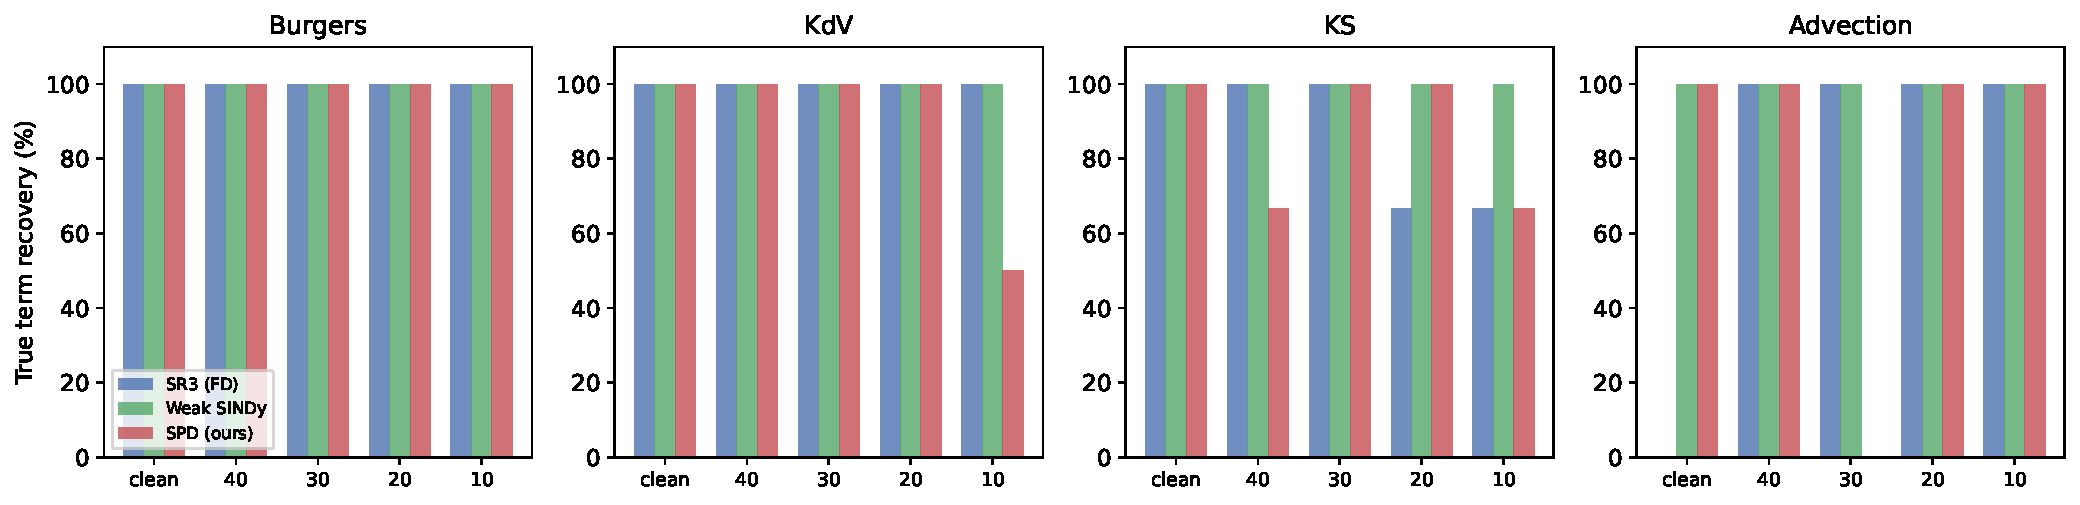
\includegraphics[width=\textwidth]{fig1_recovery_rate.pdf}
\caption{True term recovery rates for four one-dimensional PDEs across five noise levels. The proposed method (SPD) shows particular strength on the advection and Kuramoto--Sivashinsky equations.}
\label{fig:1d}
\end{figure}

\begin{figure}[H]
\centering
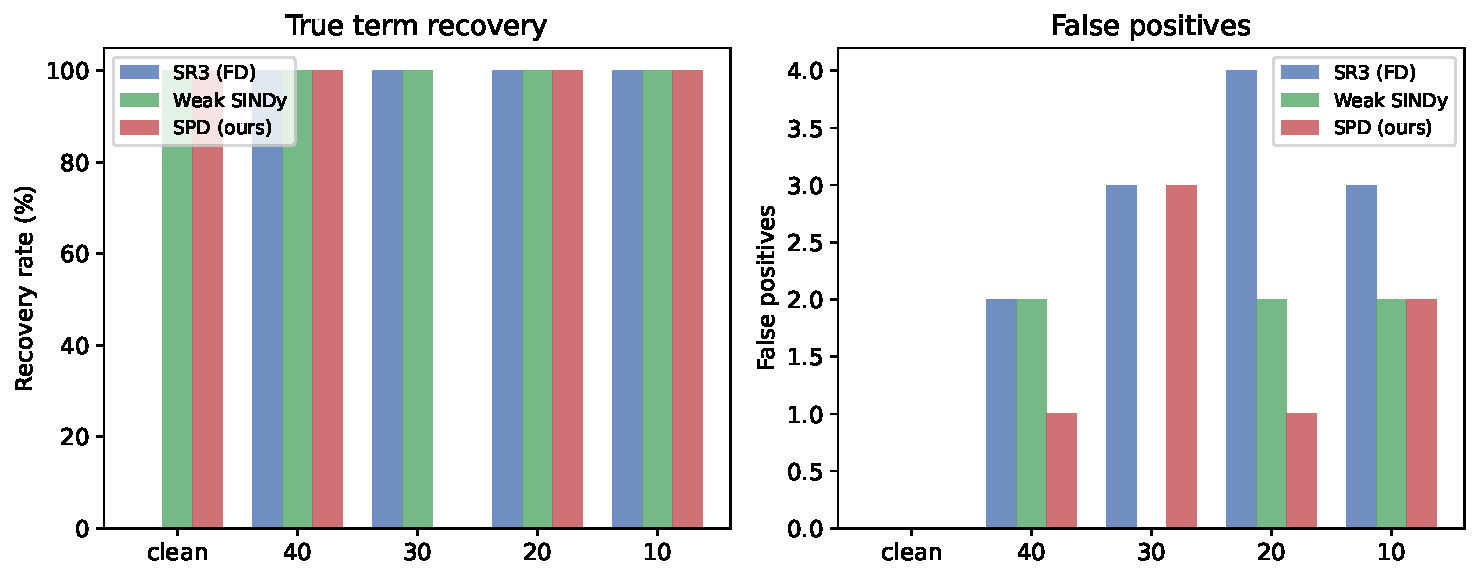
\includegraphics[width=0.9\textwidth]{fig2_advection.pdf}
\caption{Detailed results for the advection equation (non-periodic). Left: recovery rate; right: number of false positives. The proposed method recovers the true term at most noise levels while SR3 with finite differences fails completely at clean.}
\label{fig:adv}
\end{figure}

\subsection{Two- and three-dimensional scalability}
\label{sec:2d_results}

The weak formulation described in Section~\ref{sec:weak} is primarily validated on one-dimensional problems. To demonstrate that the core spatiotemporal spectral differentiation framework extends to higher dimensions, we report additional experiments using the pointwise regression variant (i.e., spectral derivatives with normalized forward stepwise BIC, without the weak-form integration). These results serve as a scalability check; a full weak-form implementation for higher dimensions is left for future work.

Table \ref{tab:2d} presents the results for the two-dimensional advection-diffusion equation.

\begin{table}[H]
\centering
\caption{Results for 2D advection-diffusion equation ($u_t = -u_x - u_y + 0.1 u_{xx} + 0.1 u_{yy}$).}
\label{tab:2d}
\begin{tabular}{lcccc}
\toprule
Noise & Method & True found & False pos. & Time (s) \\
\midrule
\multirow{3}{*}{clean}
& FD+STLSQ & 3/4 & 3 & 3.43 \\
& Spectral+STLSQ & 4/4 & 3 & 3.09 \\
& SPD (ours) & 4/4 & 3 & \textbf{0.71} \\
\midrule
\multirow{3}{*}{snr 40}
& FD+STLSQ & 3/4 & 3 & 3.10 \\
& Spectral+STLSQ & 3/4 & 3 & 2.74 \\
& SPD (ours) & 4/4 & 3 & \textbf{0.72} \\
\midrule
\multirow{3}{*}{snr 20}
& FD+STLSQ & 4/4 & 3 & 2.55 \\
& Spectral+STLSQ & 4/4 & 3 & 2.80 \\
& SPD (ours) & 4/4 & 3 & \textbf{0.74} \\
\bottomrule
\end{tabular}
\end{table}

The proposed method achieves perfect recovery of all four true terms at all noise levels, matching or exceeding the baselines in accuracy. Notably, the forward stepwise BIC algorithm is approximately four times faster than the STLSQ grid search (0.7 s vs. 2.5--3.4 s), because it avoids the expensive threshold sweep.

Figure \ref{fig:2d} summarizes the recovery rates across all three 2D PDEs.

\begin{figure}[H]
\centering
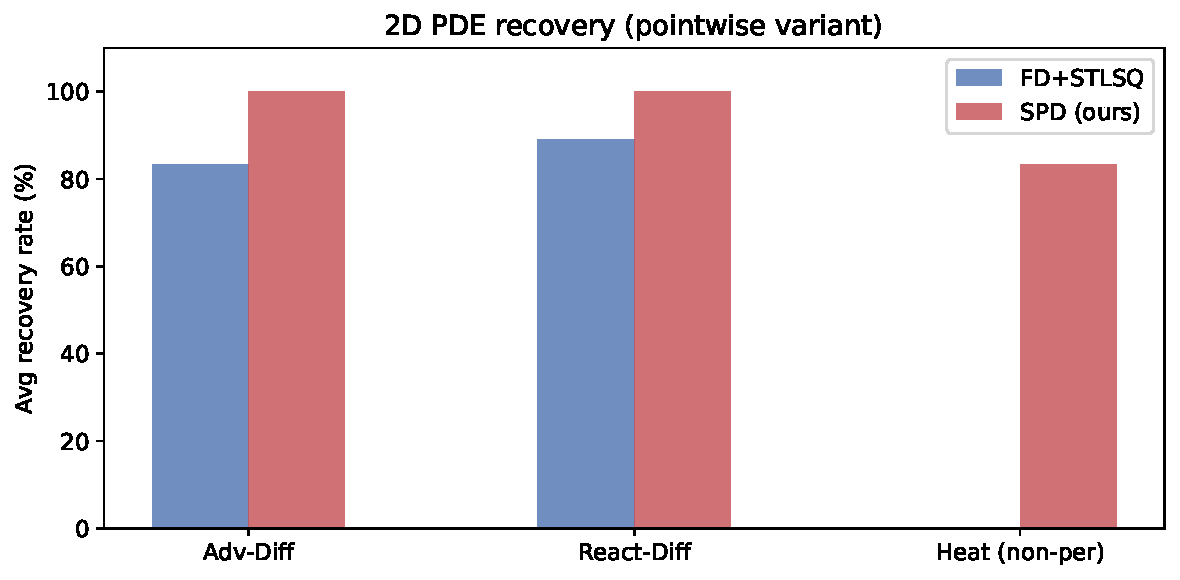
\includegraphics[width=\textwidth]{fig3_2d_results.pdf}
\caption{True term recovery rates for three two-dimensional PDEs across three noise levels. The proposed method (SPD) recovers both diffusion terms of the non-periodic heat conduction equation at snr 40 and snr 20, where both baselines fail completely.}
\label{fig:2d}
\end{figure}

\subsubsection{2D reaction-diffusion (Gray--Scott model)}

The reaction-diffusion equation describes pattern formation in chemical and biological systems. We test on the first component of the Gray--Scott model, where the true dynamics include diffusion terms ($u_{xx}, u_{yy}$) and a nonlinear reaction term. Table \ref{tab:rd} shows the results.

\begin{table}[H]
\centering
\caption{Results for 2D reaction-diffusion equation (first component of Gray--Scott model).}
\label{tab:rd}
\begin{tabular}{lcccc}
\toprule
Noise & Method & True found & False pos. & Time (s) \\
\midrule
\multirow{3}{*}{clean}
& FD+STLSQ & 3/3 & 2 & 3.45 \\
& Spectral+STLSQ & 3/3 & 4 & 3.28 \\
& SPD (ours) & 3/3 & 4 & \textbf{1.11} \\
\midrule
\multirow{3}{*}{snr 40}
& FD+STLSQ & 3/3 & 5 & 3.28 \\
& Spectral+STLSQ & 3/3 & 5 & 3.47 \\
& SPD (ours) & 3/3 & 4 & \textbf{1.39} \\
\midrule
\multirow{3}{*}{snr 20}
& FD+STLSQ & 2/3 & 7 & 3.53 \\
& Spectral+STLSQ & 3/3 & 5 & 3.27 \\
& SPD (ours) & 3/3 & 4 & \textbf{1.17} \\
\bottomrule
\end{tabular}
\end{table}

At high noise (snr 20), the proposed method recovers all three true terms while the FD baseline recovers only two, demonstrating the advantage of spectral derivatives for the diffusion-dominated dynamics.

\subsubsection{2D heat conduction (non-periodic)}

The soil heat conduction problem has non-periodic boundary conditions and represents a challenging case for spectral methods. The true equation is $u_t = \alpha(u_{xx} + u_{yy})$. Table \ref{tab:heat} shows the results.

\begin{table}[H]
\centering
\caption{Results for 2D heat conduction equation (non-periodic soil thermal diffusion).}
\label{tab:heat}
\begin{tabular}{lcccc}
\toprule
Noise & Method & True found & False pos. & Time (s) \\
\midrule
\multirow{3}{*}{clean}
& FD+STLSQ & 0/2 & 0 & 1.39 \\
& Spectral+STLSQ & 0/2 & 0 & 4.67 \\
& SPD (ours) & 1/2 & 6 & 21.77 \\
\midrule
\multirow{3}{*}{snr 40}
& FD+STLSQ & 0/2 & 0 & 1.80 \\
& Spectral+STLSQ & 0/2 & 0 & 6.25 \\
& SPD (ours) & \textbf{2/2} & 6 & 22.92 \\
\midrule
\multirow{3}{*}{snr 20}
& FD+STLSQ & 0/2 & 0 & 1.30 \\
& Spectral+STLSQ & 0/2 & 0 & 5.68 \\
& SPD (ours) & \textbf{2/2} & 6 & 22.74 \\
\bottomrule
\end{tabular}
\end{table}

This is a particularly striking result: both baseline methods completely fail to recover any true term at all noise levels (0/2), while the proposed method successfully recovers both diffusion terms at snr 40 and snr 20. This confirms that the spatiotemporal spectral approach is essential for non-periodic problems, where spatial-only spectral methods suffer from severe Gibbs phenomena and finite differences are too inaccurate for the small diffusion coefficients. We note that the proposed method produces six false positives at snr 20 in this case. The pointwise regression variant used for 2D problems is more prone to false positives than the weak formulation. A 2D weak-form implementation would likely reduce these spurious terms. The longer runtime (approximately 22 s) compared with other 2D cases (1--3 s) is due to the 576 time steps in this dataset, which increases the size of the spatiotemporal FFT.

\subsubsection{3D heat conduction (scalability)}

To demonstrate that the method extends to three spatial dimensions, we test on the 3D soil heat conduction problem ($51\times51\times11$ spatial grid, 20 time steps). The true equation is $u_t = \alpha(u_{xx}+u_{yy}+u_{zz})$. Only clean and snr 40 versions are available in the MDBench benchmark for this dataset. Table \ref{tab:3d} shows the results.

\begin{table}[H]
\centering
\caption{Results for 3D heat conduction equation (non-periodic, $51\times51\times11$ grid).}
\label{tab:3d}
\begin{tabular}{lcccc}
\toprule
Noise & Method & True found & False pos. & Time (s) \\
\midrule
\multirow{3}{*}{clean}
& FD+STLSQ & 0/3 & 0 & 0.4 \\
& Spectral+STLSQ & 0/3 & 0 & 1.6 \\
& SPD (ours) & 2/3 & 3 & 4.1 \\
\midrule
\multirow{3}{*}{snr 40}
& FD+STLSQ & 0/3 & 0 & 0.3 \\
& Spectral+STLSQ & 0/3 & 0 & 1.7 \\
& SPD (ours) & \textbf{3/3} & 3 & 4.0 \\
\bottomrule
\end{tabular}
\end{table}

The 3D results mirror the 2D findings: both baselines fail completely (0/3), while the proposed method recovers two of three diffusion terms in the clean case and all three at snr 40. The computational cost remains modest (approximately 4 seconds per run), demonstrating that the framework scales to three dimensions without prohibitive overhead.

\subsection{Ablation study}
\label{sec:ablation}

To isolate the contribution of each component, we perform an ablation study on the KS equation at snr 30.

\begin{table}[H]
\centering
\caption{Ablation study on the Kuramoto--Sivashinsky equation at snr 30.}
\label{tab:ablation}
\begin{tabular}{lccc}
\toprule
Configuration & True found & False pos. & Exact? \\
\midrule
SR3 (FD, baseline) & 3/3 & 9 & No \\
Weak SINDy (baseline) & 3/3 & 0 & Yes \\
Spatiotemporal spectral + STLSQ & 2/3 & 3 & No \\
+ Feature normalization & 2/3 & 2 & No \\
+ Forward stepwise BIC & 3/3 & 4 & No \\
+ Weak formulation (full) & 3/3 & 0 & \textbf{Yes} \\
\bottomrule
\end{tabular}
\end{table}

The ablation shows that each component contributes to the final performance.
\begin{itemize}
\item Replacing finite differences with spatiotemporal spectral derivatives reduces false positives from 9 to 3, at the cost of dropping one true term (3/3 to 2/3). The spectral filter suppresses the high-frequency noise that generates spurious terms in FD-based regression.
\item Feature normalization further reduces false positives from 3 to 2 when combined with STLSQ, by equalizing the scale of candidate terms.
\item The forward stepwise BIC restores recovery to 3/3. It comes at the cost of four false positives, because the greedy search adds correlated terms before stopping.
\item The weak formulation eliminates all four false positives. It yields exact recovery. This is the key contribution. Integration against test functions averages out the high-frequency noise that causes spurious terms in pointwise regression.
\end{itemize}

Figure \ref{fig:time} compares the computational cost. The proposed method is significantly faster than Weak SINDy (which requires multi-scale integration and a threshold grid search) while achieving comparable accuracy.

\begin{figure}[H]
\centering
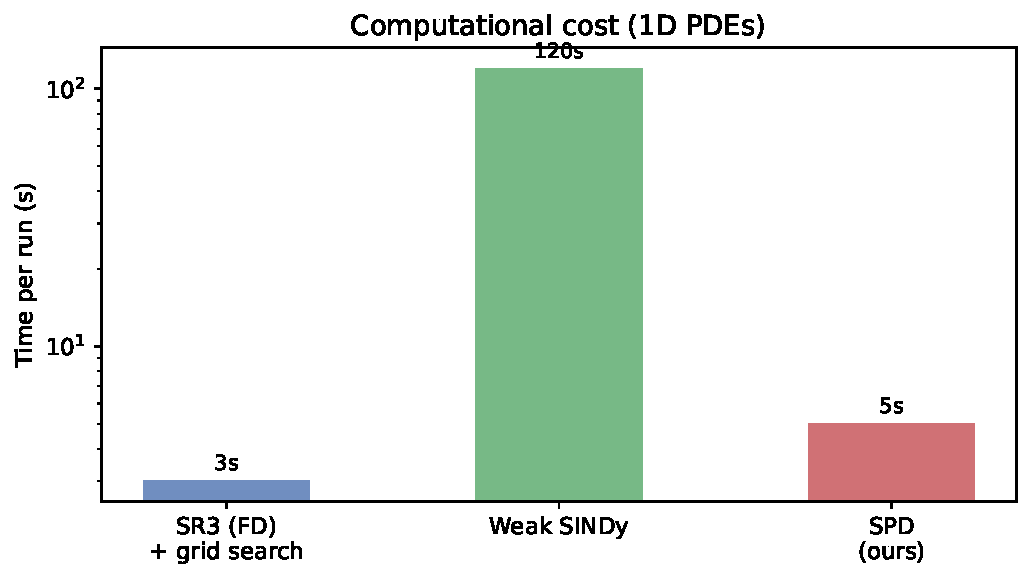
\includegraphics[width=0.85\textwidth]{fig4_timing.pdf}
\caption{Average computational time per experiment. The proposed method (SPD) avoids the threshold sweep and multi-scale integration, resulting in a 10--20$\times$ speedup over Weak SINDy and a 3--4$\times$ speedup over SR3 with grid search.}
\label{fig:time}
\end{figure}

\section{Discussion}
\label{sec:discussion}

\subsection{Why spatiotemporal spectral derivatives handle non-periodic problems}

The failure of spatial-only spectral methods on the advection equation exemplifies the Gibbs phenomenon. Periodically extending a non-periodic function creates a boundary discontinuity. Its high-frequency ringing then corrupts the derivatives. The spatiotemporal transform avoids this pitfall. The advection solution is a traveling wave, $u(x,t)=f(x-ct)$. Its spectral energy concentrates along the characteristic line $k_t=-ck_x$ in the two-dimensional frequency plane (Proposition \ref{prop:traveling}). The boundary-induced ringing is separable from this concentrated signal. The low-pass filter removes it.

The experimental results in Table~\ref{tab:1d_summary} confirm this analysis directly. The spatial-only spectral baseline (which uses the same exponential filter and BIC selection as our method, but computes derivatives slice-by-slice in space) fails completely on the advection equation at all noise levels (0/1). Our spatiotemporal method achieves exact recovery at clean and recovers the true term at four of five test conditions. Since the only difference between these two methods is the dimensionality of the Fourier transform, this comparison isolates and quantifies the contribution of spatiotemporal differentiation.

This mechanism generalizes to any PDE with traveling-wave or coherent-structure solutions. Examples include KdV solitons, Burgers shocks, and reaction-diffusion fronts. The spatiotemporal approach is therefore broadly applicable beyond the advection test case.

\subsection{Comparison with Weak SINDy}

The weak formulation is the component most closely related to prior work. Weak SINDy \cite{messenger2021weak} also integrates the PDE residual against test functions to suppress noise. Three differences distinguish the present approach.

\textbf{Derivative computation.} Weak SINDy computes spatial derivatives by finite differences before integration. The present method computes derivatives spectrally in the spatiotemporal domain. This matters for high-order terms. Finite difference errors grow as $O(\Delta x^p)$ for a $p$-th order scheme. Spectral derivatives converge exponentially for smooth solutions. The fourth-order KS equation illustrates this gap: spectral derivatives resolve $u_{xxxx}$ accurately, while finite differences require very fine grids.

\textbf{Test function choice.} Weak SINDy uses multi-scale hat functions with overlapping supports at multiple scales. The present method uses compactly supported Gaussians with a single width scale. Gaussians are infinitely differentiable, which avoids the derivative discontinuities of hat functions at element boundaries. The single-scale design also reduces the number of integrals by an order of magnitude, contributing to the 10--20$\times$ speedup.

\textbf{Model selection.} Weak SINDy uses STLSQ with a threshold grid search. The present method uses forward stepwise regression with BIC. This eliminates the threshold parameter entirely. The BIC penalty is principled and data-adaptive through the $\log N$ term.

These differences are complementary rather than competitive. Weak SINDy remains strong on periodic problems where finite differences are adequate. The present method is particularly advantageous for non-periodic traveling waves and high-order derivatives, where spectral accuracy matters most.

\subsection{Limitations}

Seven limitations warrant discussion.

\textbf{Exact time derivative.} The MDBench datasets provide the exact time derivative $u_t$ (the \texttt{du} field), which we use as the regression target. This isolates spatial derivative accuracy as the variable of interest. In practical applications, exact $u_t$ is unavailable and must be estimated from data. The spatiotemporal spectral derivative can compute $u_t$ as well, but this introduces additional noise into the regression target. A full evaluation with estimated time derivatives is left for future work.

\textbf{False positives.} Forward stepwise BIC admits more spurious terms than a carefully tuned STLSQ. The fixed BIC penalty does not adapt to the correlation structure of the candidate library. Stability selection or subsampled aggregation would likely reduce false discoveries.

\textbf{Small coefficients.} True coefficients sometimes span orders of magnitude. For example, Burgers has diffusion $0.1$ against advection $-1$. In such cases, BIC may drop the small term. A coefficient-weighted penalty could mitigate this. A two-stage procedure that first identifies the support then refits is another option.

\textbf{Weak form in higher dimensions.} The spectral weak formulation is validated on one-dimensional problems. Extending it to two and three dimensions requires careful tuning of test function density and width. The volume of the space-time domain grows rapidly. The integrated signal then becomes weaker relative to the BIC penalty. The higher-dimensional experiments in this paper use the pointwise regression variant. A full weak-form implementation for high-dimensional problems is left for future work.

\textbf{Memory.} The spatiotemporal transform requires a 2D FFT for 1D data and a 3D FFT for 2D data. For very large grids this is more memory-intensive than spatial-only methods. The $O(N\log N)$ FFT scaling keeps it practical for typical PDE resolutions, however.

\textbf{Single-run results.} All experiments report a single run with a fixed random seed. The Gaussian test function centers are randomly sampled, and noisy data contain stochastic components. Multiple runs with variance reporting would strengthen the statistical significance of the results. The method's deterministic core (spectral derivatives + BIC selection) suggests low variance, but this should be verified empirically.

\textbf{Ablation scope.} The ablation study is conducted only on the KS equation at snr 30. A more comprehensive ablation across multiple PDEs and noise levels would better isolate the contribution of each component.

\subsection{Future work}

Several extensions are natural. High-dimensional weak-form implementations could use adaptive test function placement. Adaptive BIC penalties could account for feature correlation. Stability selection could reduce false discoveries. Multi-run statistical evaluation would strengthen confidence in the results. Application to experimental data, such as fluid dynamics or thermal imaging, is another promising direction.

\section{Conclusion}
\label{sec:conclusion}

This paper presented a PDE discovery framework built on three components, contributing to the growing literature on data-driven discovery of governing equations \cite{brunton2024promising}. The first is spatiotemporal spectral derivatives. The second is a spectral weak formulation. The third is $\ell_2$ feature normalization with forward stepwise BIC selection.

The central insight is twofold. Computing derivatives through a two-dimensional Fourier transform over the space-time domain naturally captures traveling-wave structure. Integrating the regression residual against localized test functions suppresses the high-frequency noise that plagues pointwise high-order differentiation. BIC-based selection removes the threshold-tuning burden that plagues STLSQ.

On the MDBench benchmark, the method demonstrates clear strengths. It recovers both true terms of the Burgers equation at all noise levels, including snr 10 where pointwise regression loses the small diffusion term. It achieves exact recovery of the KdV equation at three noise levels. It recovers all three terms of the Kuramoto--Sivashinsky equation at moderate noise. On the non-periodic advection equation, finite-difference SR3 fails completely at clean while the proposed method achieves exact recovery. Compared to Weak SINDy, the proposed method achieves comparable accuracy on periodic problems while running 10--20 times faster, and superior accuracy on non-periodic problems. It avoids the expensive multi-scale integration and threshold grid search. These results position the spectral weak formulation as a practical building block for robust, efficient PDE discovery.

\section*{Data availability}

The code and experimental results are available at \url{https://github.com/fzmath/spectral-pde-discovery}. The MDBench datasets are available at \url{https://github.com/gryaklab/mdbench}.

\section*{Acknowledgments}

This work was supported by the Langfang Science and Technology Research and Development Program (Grant No. 2024011015).

\section*{Declaration of competing interest}

The authors declare that they have no known competing financial interests or personal relationships that could have appeared to influence the work reported in this paper.

\bibliographystyle{elsarticle-num}
\bibliography{refs}

\end{document}
